% GAMF-GAN architecture diagram (compiled standalone to figures/fig_gamf_arch.pdf)
\documentclass[border=4pt]{standalone}
\usepackage{tikz}
\usepackage{amsmath,amssymb,bm}
\usetikzlibrary{positioning,arrows.meta,fit,backgrounds,calc}
\renewcommand{\familydefault}{\sfdefault}
\begin{document}
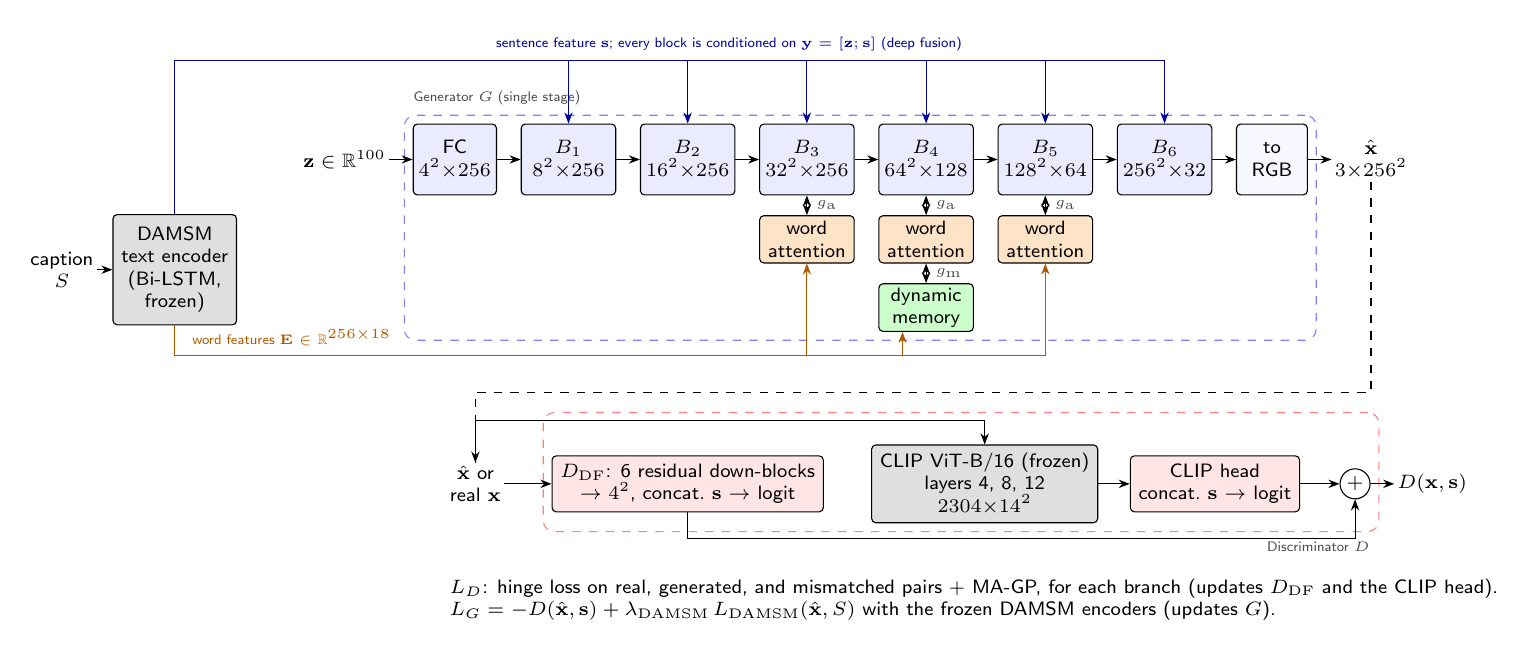
\begin{tikzpicture}[
  font=\sffamily\scriptsize, >={Stealth[length=4pt]}, node distance=3mm,
  blk/.style={draw, rounded corners=1.5pt, fill=blue!8, minimum height=9mm, minimum width=12mm, align=center, inner sep=2pt},
  att/.style={draw, rounded corners=1.5pt, fill=orange!22, minimum height=6mm, minimum width=12mm, align=center, inner sep=1.5pt},
  mem/.style={draw, rounded corners=1.5pt, fill=green!20, minimum height=6mm, minimum width=12mm, align=center, inner sep=1.5pt},
  frz/.style={draw, rounded corners=1.5pt, fill=gray!25, align=center, inner sep=3pt},
  dsc/.style={draw, rounded corners=1.5pt, fill=red!10, align=center, inner sep=3pt},
  io/.style={align=center, inner sep=1pt},
  lab/.style={font=\sffamily\tiny, text=black!70}
]
% ---------------- text encoder
\node[frz, minimum height=14mm] (txt) {DAMSM\\text encoder\\(Bi-LSTM,\\frozen)};
\node[io, left=2mm of txt] (cap) {caption\\$S$};
\draw[->] (cap) -- (txt);

% ---------------- generator
\node[io, right=8mm of txt, yshift=14mm] (z) {$\mathbf{z}\in\mathbb{R}^{100}$};
\node[blk, right=3mm of z, minimum width=9mm] (fc) {FC\\$4^2{\times}256$};
\draw[->] (z) -- (fc);
\node[blk, right=of fc] (b1) {$B_1$\\$8^2{\times}256$};
\node[blk, right=of b1] (b2) {$B_2$\\$16^2{\times}256$};
\node[blk, right=of b2] (b3) {$B_3$\\$32^2{\times}256$};
\node[blk, right=of b3] (b4) {$B_4$\\$64^2{\times}128$};
\node[blk, right=of b4] (b5) {$B_5$\\$128^2{\times}64$};
\node[blk, right=of b5] (b6) {$B_6$\\$256^2{\times}32$};
\node[blk, right=of b6, minimum width=9mm, fill=blue!3] (rgb) {to\\RGB};
\node[io, right=3mm of rgb] (x) {$\hat{\mathbf{x}}$\\$3{\times}256^2$};
\foreach \a/\b in {fc/b1,b1/b2,b2/b3,b3/b4,b4/b5,b5/b6,b6/rgb,rgb/x} \draw[->] (\a) -- (\b);

\node[att, below=2.5mm of b3] (a3) {word\\attention};
\node[att, below=2.5mm of b4] (a4) {word\\attention};
\node[mem, below=2.5mm of a4] (m4) {dynamic\\memory};
\node[att, below=2.5mm of b5] (a5) {word\\attention};
\foreach \n/\b in {a3/b3,a4/b4,a5/b5} \draw[<->] (\b) -- node[lab, right]{$g_{\mathrm{a}}$} (\n);
\draw[<->] (a4) -- node[lab, right]{$g_{\mathrm{m}}$} (m4);

% conditioning bus (sentence feature)
\coordinate (bus) at ($(b1.north)+(0,8mm)$);
\draw[->, blue!60!black] (txt.north) |- node[lab, above, pos=0.78, text=blue!60!black]{sentence feature $\mathbf{s}$; every block is conditioned on $\mathbf{y}=[\mathbf{z};\mathbf{s}]$ (deep fusion)} (b6.north|-bus) -- (b6.north);
\foreach \b in {b1,b2,b3,b4,b5} \draw[->, blue!60!black] (\b.north|-bus) -- (\b.north);
% word features
\coordinate (wbus) at ($(m4.south)+(0,-3mm)$);
\draw[->, orange!70!black] (txt.south) |- (a5.south|-wbus) -- (a5.south);
\node[lab, text=orange!70!black, anchor=south west] at ($(txt.south|-wbus)+(1mm,0)$) {word features $\mathbf{E}\in\mathbb{R}^{256\times18}$};
\draw[->, orange!70!black] (a3.south|-wbus) -- (a3.south);
\coordinate (m4w) at ($(m4.south)+(-3mm,0)$);
\draw[->, orange!70!black] (m4w|-wbus) -- (m4w);

\begin{scope}[on background layer]
\node[draw=blue!50, dashed, rounded corners, fit=(fc)(b6)(rgb)(a3)(m4)(a5), inner sep=3pt, label={[lab, anchor=south west]north west:Generator $G$ (single stage)}] (Gbox) {};
\end{scope}

% ---------------- discriminator
\node[dsc, below=33mm of b2, minimum width=30mm] (ddf) {$D_{\mathrm{DF}}$: 6 residual down-blocks\\$\to 4^2$, concat.\ $\mathbf{s}$ $\to$ logit};
\node[frz, right=6mm of ddf] (clip) {CLIP ViT-B/16 (frozen)\\layers 4, 8, 12\\$2304{\times}14^2$};
\node[dsc, right=4mm of clip] (chead) {CLIP head\\concat.\ $\mathbf{s}$ $\to$ logit};
\node[circle, draw, inner sep=1pt, right=5mm of chead] (sum) {$+$};
\node[io, right=3mm of sum] (dout) {$D(\mathbf{x},\mathbf{s})$};
\draw[->] (clip) -- (chead);
\draw[->] (chead) -- (sum);
\draw[->] (ddf.south) |- ($(sum.south)+(0,-5mm)$) -- (sum.south);
\draw[->] (sum) -- (dout);
\node[io, left=6mm of ddf] (xin) {$\hat{\mathbf{x}}$ or\\real $\mathbf{x}$};
\draw[->] (xin) -- (ddf);
\coordinate (cr) at ($(clip.north)+(0,3mm)$);
\draw[->] (xin.north) |- (cr) -- (clip.north);
\coordinate (route) at ($(ddf.north)+(0,8mm)$);
\draw[->, dashed] (x.south) |- (xin.north|-route) -- (xin.north);
\begin{scope}[on background layer]
\node[draw=red!50, dashed, rounded corners, fit=(ddf)(clip)(chead)(sum)(cr), inner sep=3pt, label={[lab, anchor=north east]south east:Discriminator $D$}] {};
\end{scope}

% ---------------- losses
\node[io, align=left, anchor=north west] at ($(xin.west|-ddf.south)+(0,-8mm)$) {%
$L_D$: hinge loss on real, generated, and mismatched pairs + MA-GP, for each branch (updates $D_{\mathrm{DF}}$ and the CLIP head).\\
$L_G = -D(\hat{\mathbf{x}},\mathbf{s}) + \lambda_{\mathrm{DAMSM}}\,L_{\mathrm{DAMSM}}(\hat{\mathbf{x}},S)$ with the frozen DAMSM encoders (updates $G$).};
\end{tikzpicture}
\end{document}
